\documentclass[a4paper]{article}
\usepackage{amssymb}
\usepackage{amsmath}
\usepackage{hyperref}
\usepackage[italian]{cleveref}
\usepackage[autostyle=false, style=english]{csquotes}
\usepackage[italian]{babel}
%\usepackage[nomarkers]{endfloat}
\usepackage{graphicx}
\usepackage[margin=3cm]{geometry}
\usepackage{mathtools}
\usepackage{parskip}
\usepackage{subcaption}
\usepackage[table]{xcolor}
\usepackage[math]{cellspace}
\cellspacetoplimit 4pt
\cellspacebottomlimit 4pt
%\renewcommand{\efloatseparator}{\mbox{}}
%\renewcommand{\efloatendlist}{\mbox{}}
\newenvironment{eqsys}{\begin{equation}\begin{dcases}}{\end{dcases}\end{equation}}
\graphicspath{{./images/}}
\MakeOuterQuote{"}

\DeclareMathOperator*{\sca}{\textrm{sca}}
\title{Progetto Controlli Automatici T \\ 1C - Controllo del posizionamento di un link flessibile}
\author{Riccardo Corradini \and Luigi di Nuzzo \and Kevin Michael Frick \and Davide Ragazzini \and Antony Zappacosta}
\begin{document}
\maketitle
\tableofcontents
\clearpage
\section{Descrizione e requisiti del sistema}
Nella nuova applicazione della azienda che commissiona il progetto si prevede di utilizzare una struttura meccanica particolarmente leggera.
Questa però presenta il problema di una flessibilità non trascurabile intrinseca nei componenti meccanici utilizzati.
Ciò rende difficile il posizionamento dell’estremità non attuata in una posizione fissa desiderata.
\subsection{Modello e linearizzazione}
L’intera struttura in questione è modellizzata dalla \cref{eqn:model} ed è schematizzata come in \cref{fig:sys_schem}.
\begin{eqsys}
    \label{eqn:model}
    \dot{x_1}  =  f_1 (x_1, x_2, x_3, x_4, u)  =  x_2 \\
    \dot{x_2}  =  f_2 (x_1, x_2, x_3, x_4, u)  =  \frac{-M g L \sin (x_1) - K (x_1 - x_3) - \rho (x_2 - x_4)}{J} \\
    \dot{x_3}  =  f_3 (x_1, x_2, x_3, x_4, u)  =  x_4 \\
    \dot{x_4}  =  f_4 (x_1, x_2, x_3, x_4, u)  =  \frac{K(x_1 - x_2) + \rho (x_2 - x_4) + u}{I}\\
    y  =  f_y (x_1, x_2, x_3, x_4)  =  x_1
\end{eqsys}
\begin{figure}[h!]
    \centering
 \begin{subfigure}{0.45\textwidth}
    \centering
    \includegraphics[width=\textwidth]{schematic.png}
    \caption{Schema del modello fisico del sistema.}
    \label{fig:sys_schem}
 \end{subfigure}
 ~
 \begin{subfigure}{0.45\textwidth}
    \centering
    \includegraphics[width=\textwidth]{control_sys.png}
    \caption{Schema di controllo del sistema linearizzato.}
    \label{fig:sys_cont}
 \end{subfigure}
\end{figure}
La variabile $\theta$ in \cref{fig:sys_schem} viene descritta dallo stato $x_1$ e rappresenta l’angolo rispetto ad un piano di riferimento fisso che la massa concentrata del link traccia nel suo moto. $\theta_m$ (nelle equazioni $x_3$) rappresenta l’angolo di rotazione del motore, il cui input $u$ al sistema è la coppia applicata $\tau_m$. $K, \rho, L, M_p, J_p, I$ sono rispettivamente: la costante elastica del link, il suo coefficiente di attrito dinamico, la lunghezza, la massa concentrata sull’estremità non attuata, il momento d’inerzia della stessa massa e il momento d’inerzia del link equivalente visto dal punto di vista del motore.
Ai fini dello sviluppo del controllo dell’impianto si vuole ottenere la struttura in \cref{fig:sys_cont}.

Come prima analisi il sistema non lineare è stato considerato nell’intorno di un punto di equilibrio, i cui valori $(\bar{x}, \bar{u})$ sono definiti nella \cref{table:ref_val}, e linearizzato nello stesso intorno servendosi della \cref{table:linearization_calc} ottenendo la \cref{eqn:linearization} e il sistema nella \cref{eqn:linearized}.
Si è passato poi dalla rappresentazione nello spazio degli stati al dominio di Laplace utilizzando la trasformata di Laplace, ottenendo la funzione di trasferimento nella \cref{eqn:G}.

{\begin{table}[h!]

    \centering

    \rowcolors{1}{gray!10}{gray!20}
    \begin{tabular}{| c | c || c | c |}

        $K$ & 3 &
        $\rho$ & 0.2 \\
        $L$ & 1 &
        $I$ & 0.01 \\
        $J_p$ & 0.02 &
        $M_p$ & 0.06 \\
        $\omega_n$ & 200 &
        $A_n$ & 0.05 \\
        $B_n$ & 20 &
        $h\%$ & 1 \\
        $T_{a_{h^\%}}$ & 0.8 &
        $W$ & $5^\circ$ \\
        $T_{a_o}$ & 0.4 &
        $\bar{u}$  & $M_p g L \sin(\bar{x_1})$ \\
        $\bar{x_1}$  & $\frac{\pi}{2}$ &
        $\bar{x_2}$  & 0 \\
        $\bar{x_3}$  &$\frac{\bar{u}}{K} + \bar{x_1}$ &
        $\bar{x_4}$  & 0


    \end{tabular}
    \caption{Specifiche del sistema.}
        \label{table:ref_val}
\end{table}
}

{\begin{table}[h]

\centering

    \rowcolors{1}{gray!10}{gray!20}
    \begin{tabular}{| Sc | Sc | Sc | Sc |}

\(\displaystyle \frac{\partial f_1}{\partial x_1} = 0 \) &
\(\displaystyle \frac{\partial f_1}{\partial x_2} = 1\) &
\(\displaystyle \frac{\partial f_1}{\partial x_3} = 0\) &
\(\displaystyle \frac{\partial f_1}{\partial x_4} = 0 \)\\
\(\displaystyle \frac{\partial f_2}{\partial x_1} = \frac{(-M_p g L \cos(x_1) - K)}{J_p}\) &
\(\displaystyle \frac{\partial f_2}{\partial x_2} = \frac{-\rho}{J_p}\) &
\(\displaystyle \frac{\partial f_2}{\partial x_3} = \frac{K}{J_p}\) &
\(\displaystyle \frac{\partial f_2}{\partial x_4} = \frac{\rho}{J_p} \)\\
\(\displaystyle \frac{\partial f_3}{\partial x_1} = 0\) &
\(\displaystyle \frac{\partial f_3}{\partial x_2} = 0\) &
\(\displaystyle \frac{\partial f_3}{\partial x_3} = 0\) &
\(\displaystyle \frac{\partial f_3}{\partial x_4} = 1 \)\\
\(\displaystyle \frac{\partial f_4}{\partial x_1} = \frac{K}{I}\) &
\(\displaystyle \frac{\partial f_4}{\partial x_2} = \frac{\rho}{I}\) &
\(\displaystyle \frac{\partial f_4}{\partial x_3} = -\frac{K}{I}\) &
\(\displaystyle \frac{\partial f_4}{\partial x_4} = -\frac{\rho}{I} \)\\
\(\displaystyle \frac{\partial f_1}{\partial u} = 0\) &
\(\displaystyle \frac{\partial f_2}{\partial u} = 0\) &
\(\displaystyle \frac{\partial f_3}{\partial u} = 0\) &
\(\displaystyle \frac{\partial f_4}{\partial u} = \frac{1}{I} \)\\
\(\displaystyle \frac{\partial f_y}{\partial x_1} = 1\) &
\(\displaystyle \frac{\partial f_y}{\partial x_2} = 0\) &
\(\displaystyle \frac{\partial f_y}{\partial x_3} = 0\) &
\(\displaystyle \frac{\partial f_y}{\partial x_4} = 0 \)
\end{tabular}
\caption{Linearizzazione del sistema.}
\label{table:linearization_calc}
\end{table}}

\begin{equation}
    \label{eqn:linearization}
A = \begin{pmatrix}0 & 1 & 0 & 0 \\
    -K/J_p & -\rho/J_p & K/J_p & \rho/J_p \\
    0    &   0    &   0    &   1\\
    K/I  & \rho/I & -K/I &-\rho/I
\end{pmatrix};
B = (0, 0, 0, \frac{1}{I})^T;
C = (1, 0, 0, 0);
D = (0);
\end{equation}

\begin{eqsys}
\label{eqn:linearized}
\delta \dot{x} = A \delta x + B \delta u\\
\delta y = C \delta x + D \delta u
\end{eqsys}




\begin{equation}
    \label{eqn:G}
    G(s) = \frac{1000 (s+15)}{s^2 (s^2 + 30s + 450)}
\end{equation}
Dopo aver definito su MATLAB i parametri del sistema, le matrici corrispondenti alla rappresentazione nello spazio degli stati del sistema linearizzato e la sua funzione di trasferimento, si è tracciato il diagramma di Bode del sistema in anello aperto, mostrato in \cref{fig:bode_G}, per $\omega \in [10^{-2}, 10^5]$.

\begin{figure}[h!]
    \centering
    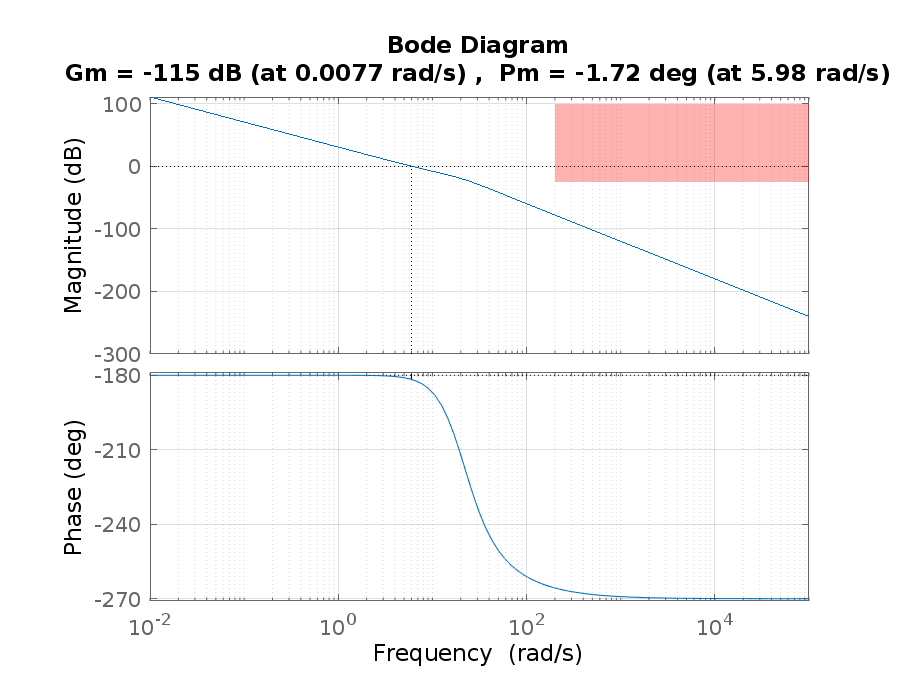
\includegraphics[width=\textwidth]{bode_G}
    \caption{Diagramma di Bode del sistema in anello aperto.}
    \label{fig:bode_G}
\end{figure}

\subsection{Specifiche}
Per l’applicazione che l’azienda ha in mente si devono rispettare per il sistema linearizzato determinate caratteristiche:
\begin{enumerate}
    \item Errore a regime nullo con riferimento a gradino con ampiezza $w(t) = W \sca(t)$.
    \item Margine di fase $\phi_m \geq 45^\circ$.
    \item Sovraelongazione percentuale $S\% \leq 1\%$.
    \item Tempo di assestamento all'1\% $T_{a1} = 0.8\hspace{0.3em} [s]$ (opzionalmente $0.4 \hspace{0.3em}[s]$).
    \item Abbattimento di 20 volte di un disturbo di misura che si fa sentire a $\omega_n > 200\hspace{0.3em} [rad/s]$ con ampiezza $A_n = 0.05$.
\end{enumerate}

\subsection{Requisiti sul margine di fase e sulla pulsazione critica}
Il requisito sulla sovraelongazione si traduce in un requisito sul margine di fase che è maggiore di quello specificato, indicato nella \cref{eqn:phim}.
Tuttavia, durante la sintesi del controllore si è notato che anche non rispettando questo requisito è possibile avere un sistema che rispetti le specifiche di sovraelongazione e abbia un tempo di assestamento ottimale.
Nei diagrammi di Bode l'intervallo che comprende fasi non accettabili, pur rispettando le specifiche sul tempo di assestamento e sull'abbattimento del rumore, è indicato in blu.

\begin{equation}
    \xi = \sqrt{\frac{\log(S_{max})^2}{(\pi^2+\log(S_{max})^2)}} \approx 0.826
    \label{eqn:xi}
\end{equation}

\begin{equation}
    \phi_m \approx \xi \cdot 100 \approx 83^\circ
    \label{eqn:phim}
\end{equation}

Il requisito sul tempo di assestamento si traduce invece in un requisito sulla pulsazione critica, che deve essere maggiore di una certa soglia indicata nella \cref{eqn:omega_c}.
Questa soglia è stata rispettata durante la sintesi del regolatore.
Nei diagrammi di Bode le "zone proibite" che non rispettano i requisiti sono indicate in verde; le specifiche ottimali usano un colore meno intenso.
\begin{equation}
    \omega_c \gtrsim \frac{460}{\phi_m T_a} \approx 7 \hspace{0.3em} [rad/s] (\approx 14 \hspace{0.3em} [rad/s] \textrm{ per le specifiche ottimali})
    \label{eqn:omega_c}
\end{equation}

\section{Progetto del regolatore}

Per avere errore a regime nullo è necessario che $L(s)$ abbia un polo nell'origine, ma $G(s)$ ne ha due, che abbassano di molto la fase: si progetta quindi $R(s)$ in modo che abbia uno zero vicino all'origine che cancelli il polo.

\subsection{Specifiche standard}
Per rispettare le specifiche standard si è inserito uno zero nell'origine per cancellare un polo di $G(s)$ e avere un margine di fase pari ad almeno 83 gradi per pulsazioni critiche $\omega_c \le 10\hspace{0.3em} rad/s$.
Si è quindi cercato un guadagno che permettesse di rispettare tale pulsazione critica, dato dalla \cref{eqn:gain}.
\begin{equation}
\mu_d =  10^{-\frac{1}{20}|(s \cdot G)(j \bar{\omega}_c)|_{dB}} \approx 0.38, \bar{\omega}_c = 16 \hspace{0.3em} [rad/s]
\label{eqn:gain}
\end{equation}
Si è quindi inserito un polo a quattro decadi dall'origine per garantire la fisica realizzabilità.
Si è osservato che, nonostante non si stessero rispettando le specifiche sul margine di fase, il sistema presenta comunque una sovraelongazione estremamente ridotta.
La funzione di trasferimento del regolatore è data dalla \cref{eqn:R}.
Il diagramma di Bode è mostrato in \cref{fig:bode_L}.
\begin{equation}
    \label{eqn:R}
    R(s) = \frac{ 0.38 s}{ 1+  10^{-4} s}
\end{equation}

\begin{figure}[h!]
    \centering
    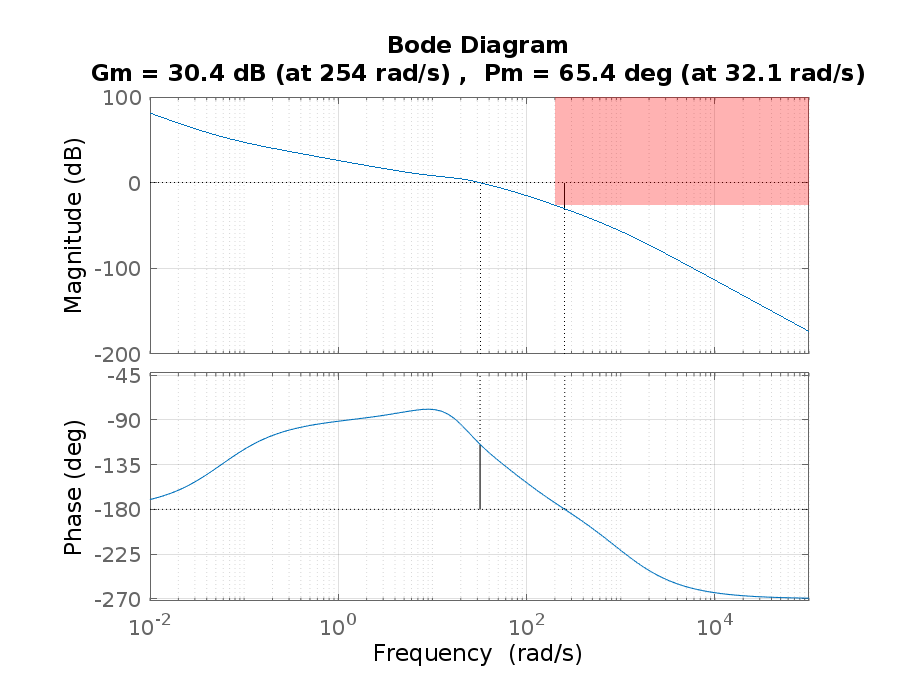
\includegraphics[width=\textwidth]{bode_L}
    \caption{Diagramma di Bode del sistema con regolatore.}
    \label{fig:bode_L}
\end{figure}


\section{Risposta del sistema in anello chiuso con regolatore}
Il regolatore garantisce un tempo di assestamento all'1\% pari a 393 millisecondi (misurato con la funzione MATLAB \texttt{stepinfo}).
\begin{figure}[h!]
    \centering
    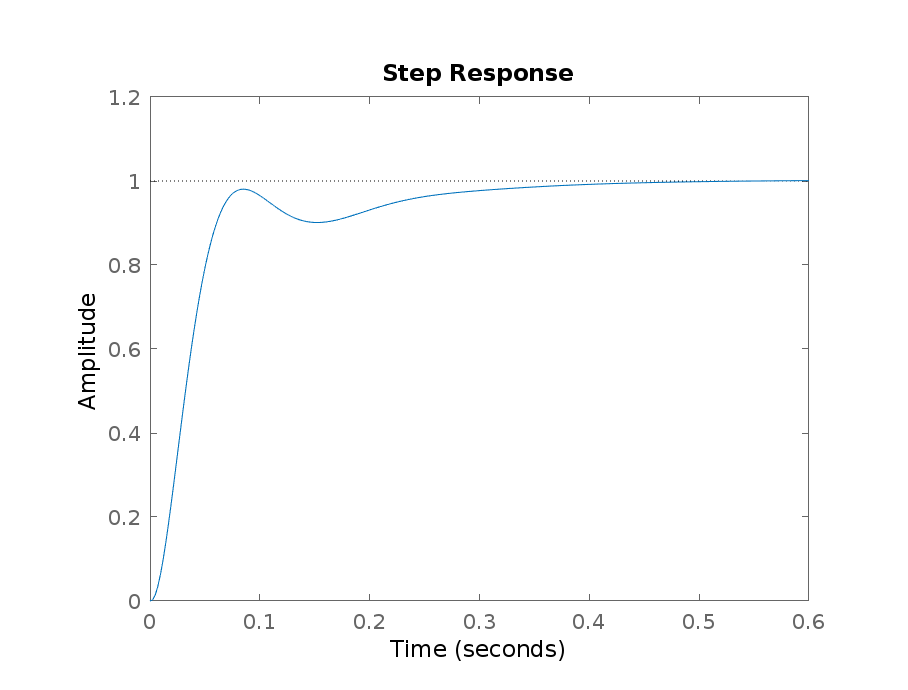
\includegraphics[width=0.8\textwidth]{step}
    \caption{Risposta allo scalino del sistema in anello chiuso con regolatore.}
    \label{fig:step}
\end{figure}

\subsection{Studio del luogo delle radici}
Dallo studio del luogo delle radici mostrato in \cref{fig:rlocus} si evince che i poli nell'origine tendono a diventare complessi coniugati a parte reale positiva per valori alti della costante di trasferimento.
Ciò significa che aumentando il guadagno il sistema diventa instabile.
Con il regolatore progettato, tuttavia, il guadagno non è abbastanza alto perché ciò accada.
Si osserva inoltre che i poli dominanti rispettano i requisiti sulla parte reale dati dalle specifiche sul tempo di assestamento, ma non quelli sullo smorzamento dati dalle specifiche sulla sovraelongazione.

\begin{figure}[h!]
    \centering
    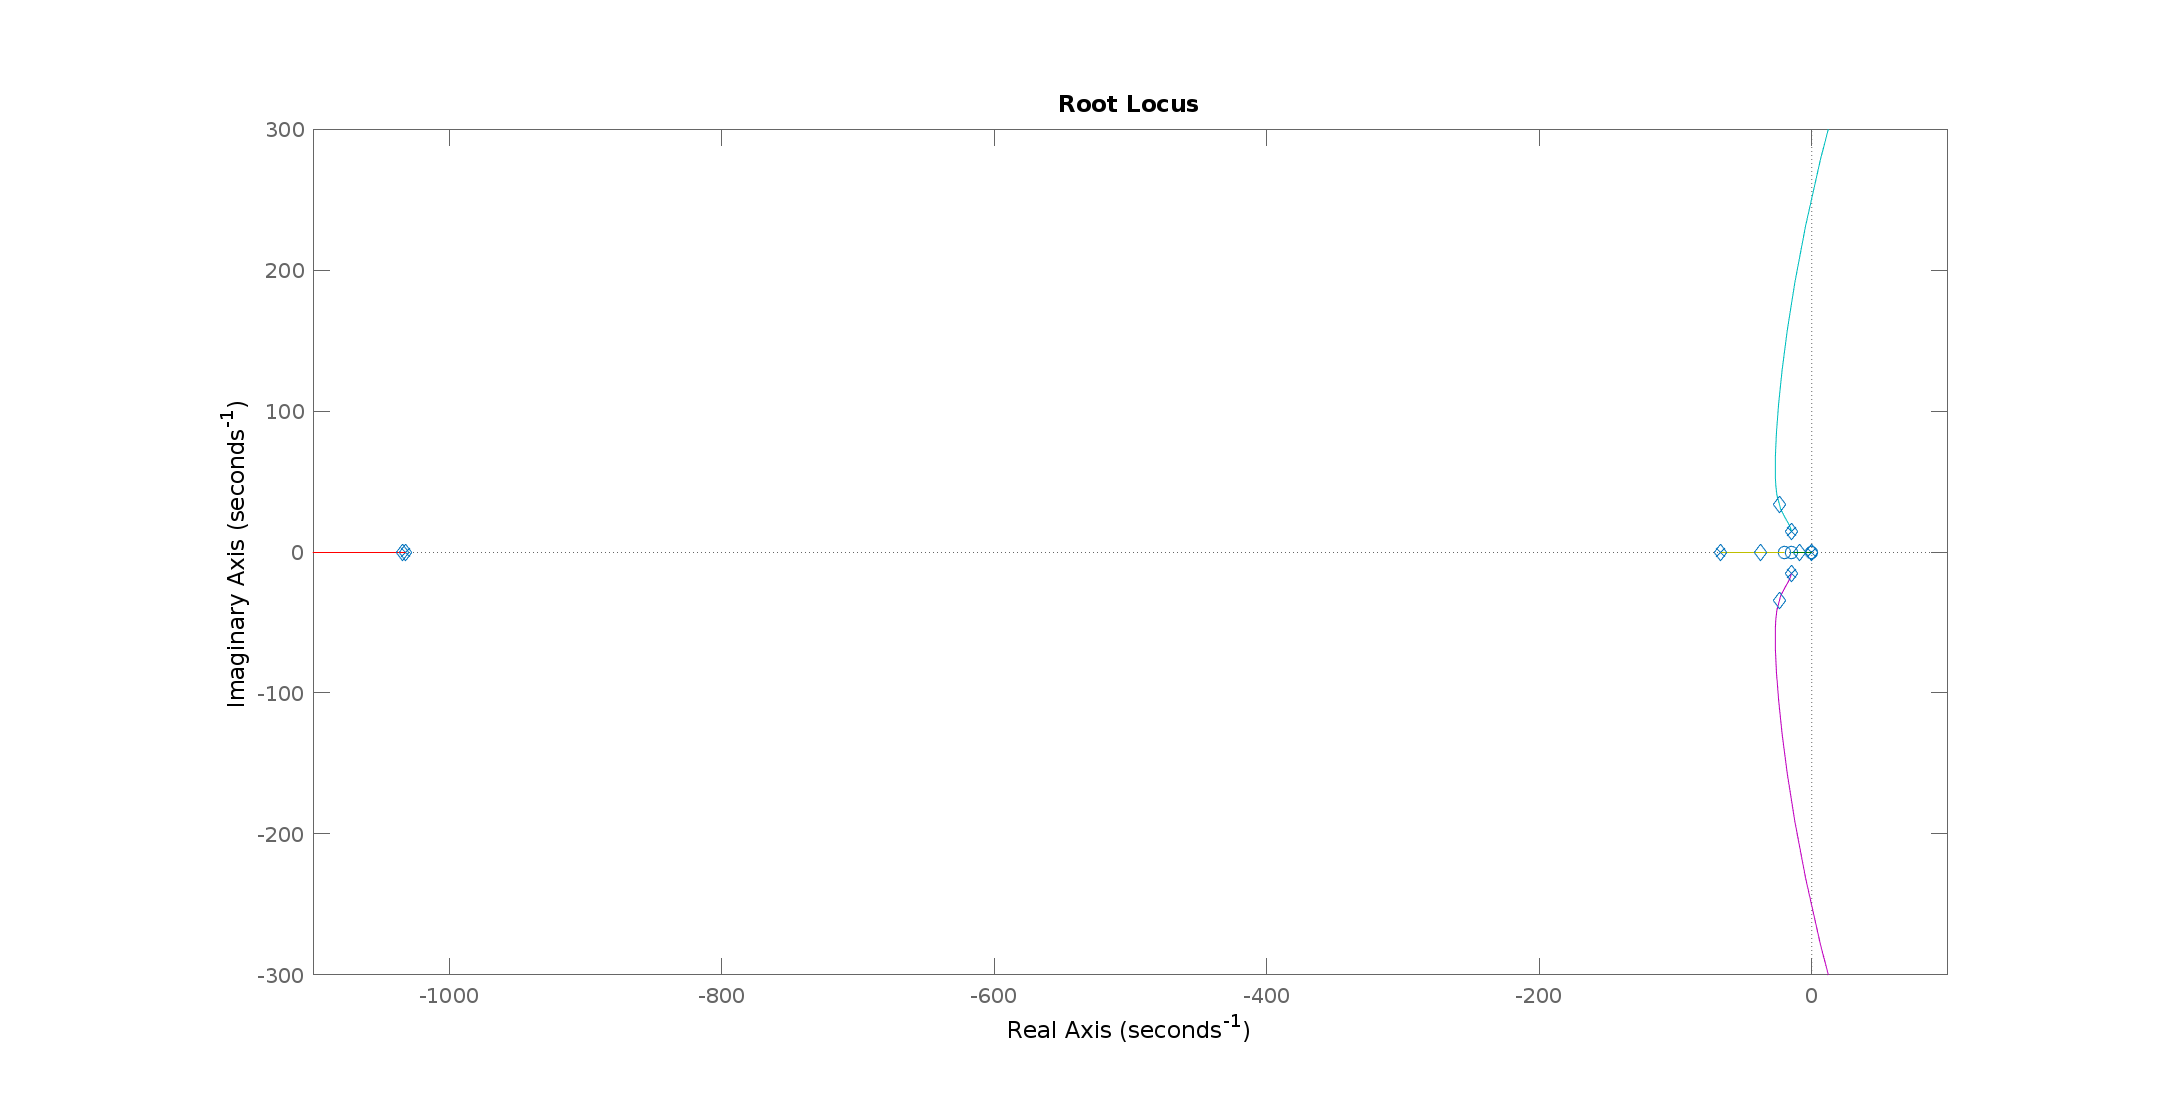
\includegraphics[width=0.65\textwidth]{rlocus}
    \caption{Luogo delle radici del sistema con regolatore.}
    \label{fig:rlocus}
\end{figure}

\subsection{Simulink}
Il sistema è stato simulato, sia nella sua versione linearizzata che in quella non linearizzata, servendosi del pacchetto software Simulink.
Il sistema non linearizzato è stato realizzato con un blocco "MATLAB Function" che calcola le espressioni nella \cref{eqn:model}, le passa a quattro blocchi integratori e riceve in ingresso il risultato.
Si osserva tuttavia che il sistema non linearizzato presenta notevoli divergenze dal sistema linearizzato per i valori di ingresso a scalino richiesti dalle specifiche, rimanendo stabile solo con sollecitazioni almeno mille volte meno intense.
\begin{figure}[h!]
    \centering
    \includegraphics[width=0.7\textwidth]{Simul1C.pdf}
    \caption{Schema Simulink del sistema linearizzato.}
    \label{fig:sim_lin}
\end{figure}
\begin{figure}[h!]
    \centering
    \includegraphics[width=0.7\textwidth]{NonLin1C.pdf}
    \caption{Schema Simulink del sistema non linearizzato. }
    \label{fig:sim_nonlin}
\end{figure}
La risposta allo scalino del sistema linearizzato ricalca quella ottenuta con la funzione \texttt{step} di MATLAB.
La risposta allo scalino del sistema non linearizzato mostra che è possibile ottenere stabilità solamente con valori di ingresso a scalino inferiori a $w = \frac{W}{1000} \sca(t)$.
\section{Conclusioni}
Nonostante le buone prestazioni ottenute dal regolatore sul sistema linearizzato, il sistema reale è resistente solo a sollecitazioni mille volte minori del riferimento.
Le specifiche sulla sovraelongazione sembrano richiedere un margine di fase più ampio di quello fornito dal regolatore ottimale, nondimeno si osserva come quest'ultimo non presenti sovraelongazione.
Queste criticità mettono in evidenza l'entità delle approssimazioni utilizzate durante la sintesi del sistema di controllo e dovrebbero essere portate all'attenzione dell'azienda che commissiona il progetto e attentamente esaminate prima della fisica realizzazione e installazione del regolatore.
\begin{figure}[h]
    \centering
    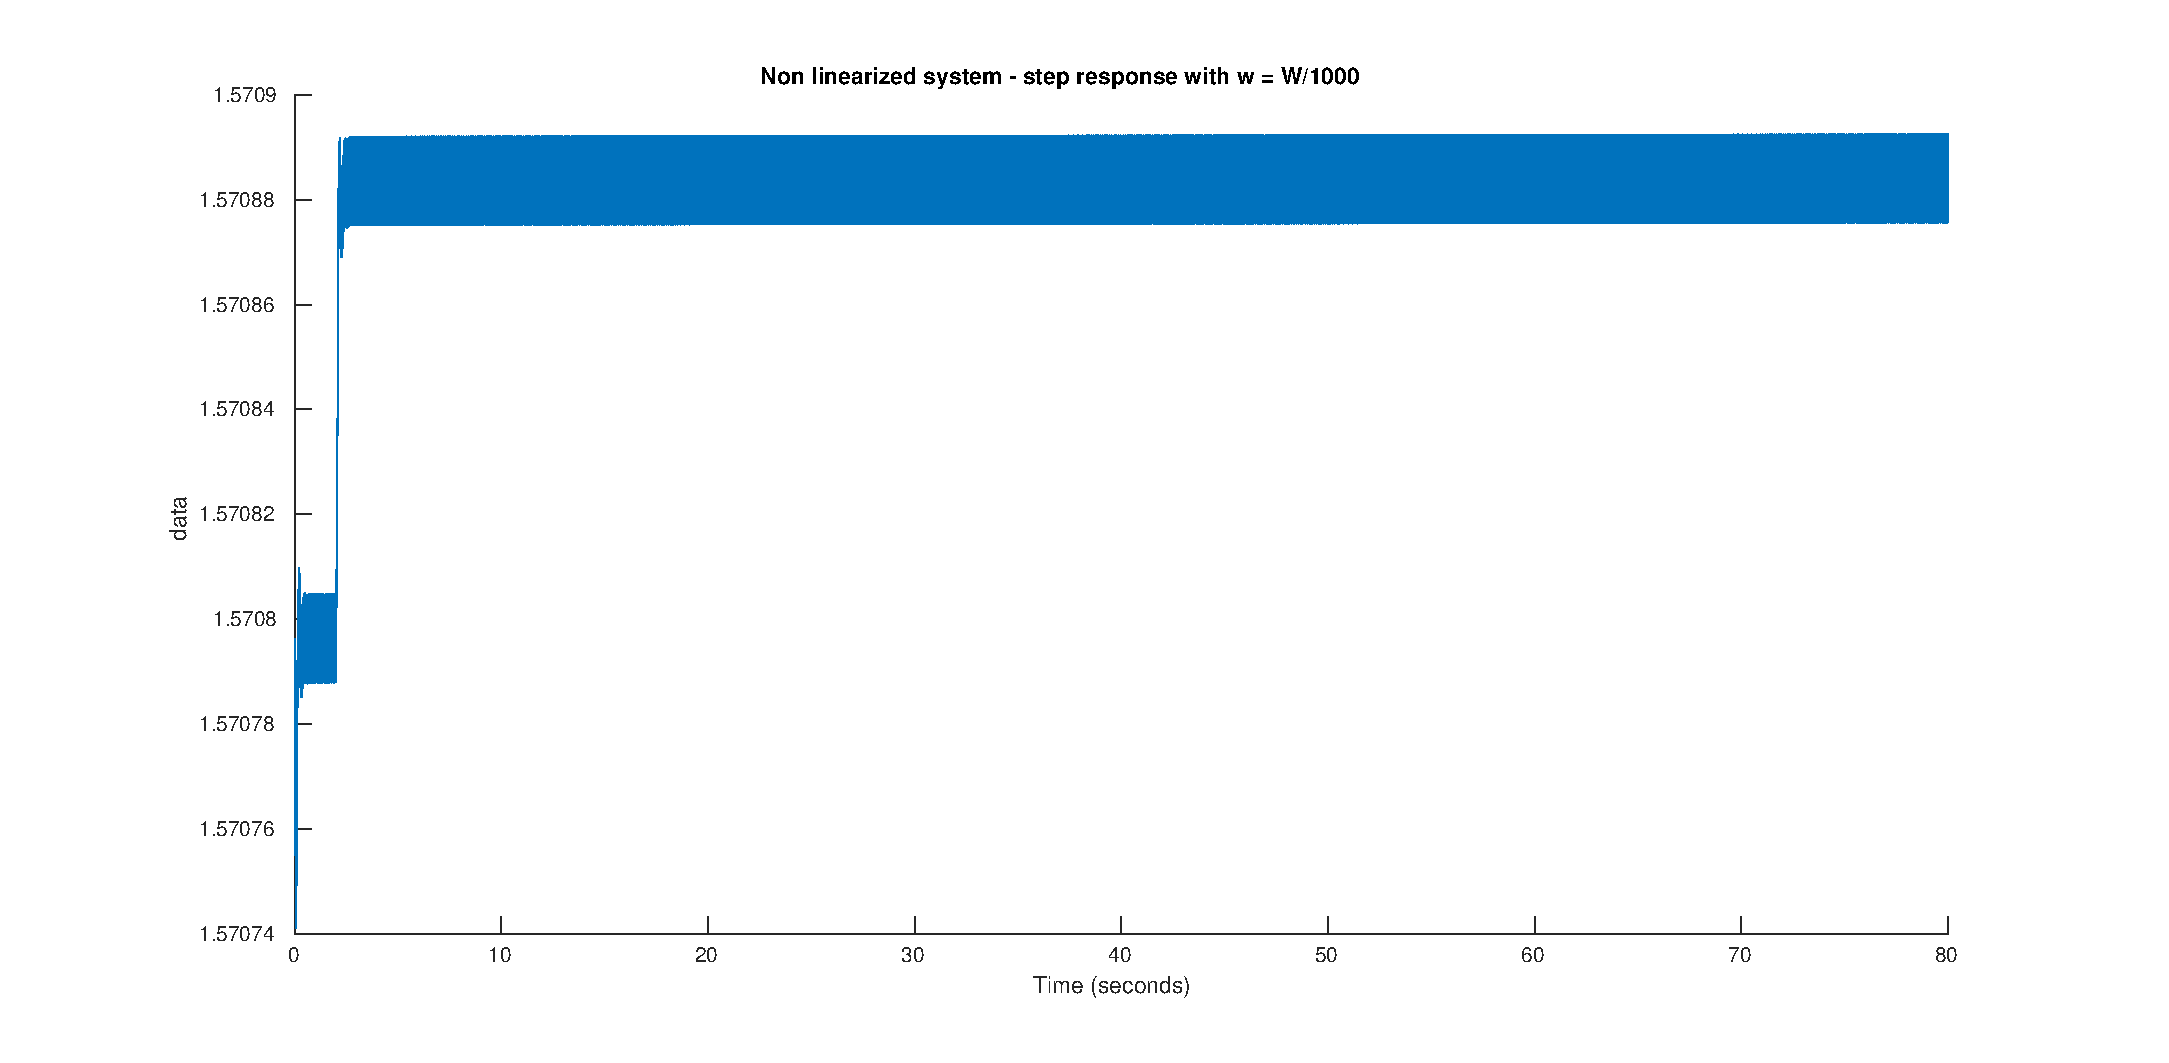
\includegraphics[width=0.7\textwidth]{step_nonlin_long}
    \caption{Risposta allo scalino del sistema non linearizzato con ingresso $w = \frac{W}{1000} \sca (t)$.}
    \label{fig:step_sim_nonlin_long}
\end{figure}

\end{document}
